% This is text associated with the open textbook "Open Electromagnetics"
% See immediately below for author, date
% This work is licensed under the Creative Commons Attribution-ShareAlike 4.0 International License. (CC BY-SA 4.0) 
% To view a copy of the license, visit http://creativecommons.org/licenses/by-sa/4.0/

%ORB TITLE Coordinate Systems
%ORB AUTHOR 0        # S.W. Ellingson, Virginia Tech (ellingson@vt.edu)
%ORB DATE 20191113   # yyyymmdd
%ORB ABSTRACT 

\label{m0180_Coordinate_Systems} % <-- Must match name of this file and module directory name.  Don't mess with this!

The coordinate systems most commonly used in engineering analysis are the \emph{Cartesian}, \emph{cylindrical}, and \emph{spherical} systems.
These systems are illustrated in Figures~\ref{m0180_fCartesianBasis}, \ref{m0180_fCylindricalCoordinates}, and \ref{m0180_fSphericalCoordinates}, respectively.
Note that the use of variables is not universal; in particular, it is common to encounter the use of $r$ in lieu of $\rho$ for the radial coordinate in the cylindrical system, and the use of $R$ in lieu of $r$ for the radial coordinate in the spherical system.
%
\begin{figure}[b!]
\begin{center}
\pdftooltip{{  % note double braces
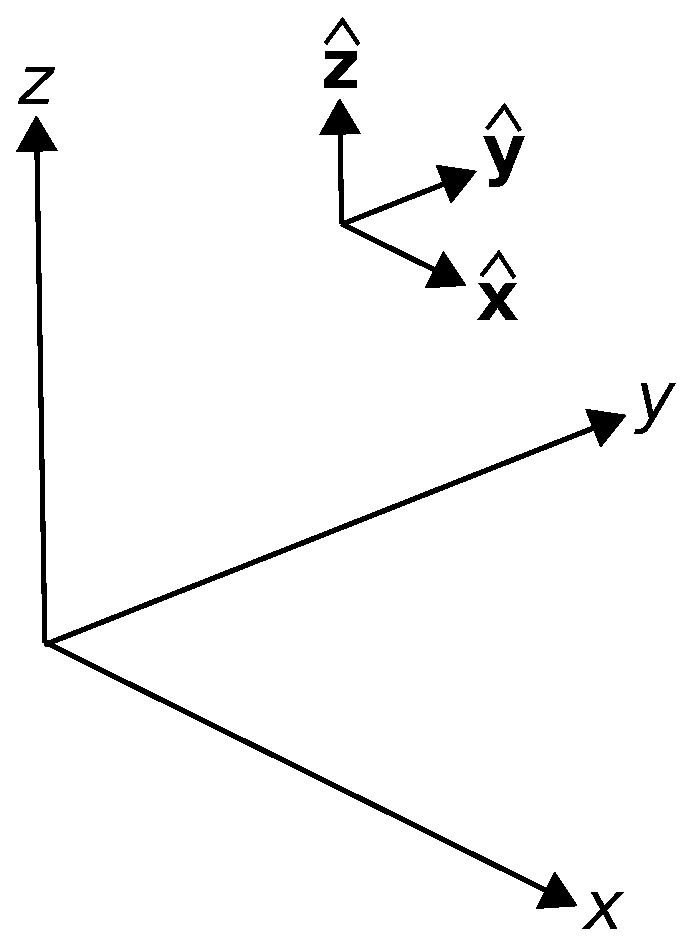
\includegraphics[width=1.5in]{modules/m0180_fCartesianBasis.eps}
% https://commons.wikimedia.org/wiki/File:m0006_fCartesianBasis.svg
}}{Shows the Cartesian coordinate system. Overlayed on this are basis vectors x-hat, y-hat, and z-hat corresponding to the axes of the coordinate system.}
\end{center} 
\centerline{\scriptsize 
\copyright~\hyperref[m0180_fCartesianBasis_Credit]{K.\ Kikkeri} 
\href{https://creativecommons.org/licenses/by-sa/4.0/}{CC BY~SA 4.0} 
} 
\caption{
\label{m0180_fCartesianBasis}
Cartesian coordinate system.
}
\end{figure}
%
\begin{figure}
\begin{center}
\pdftooltip{{  % note double braces
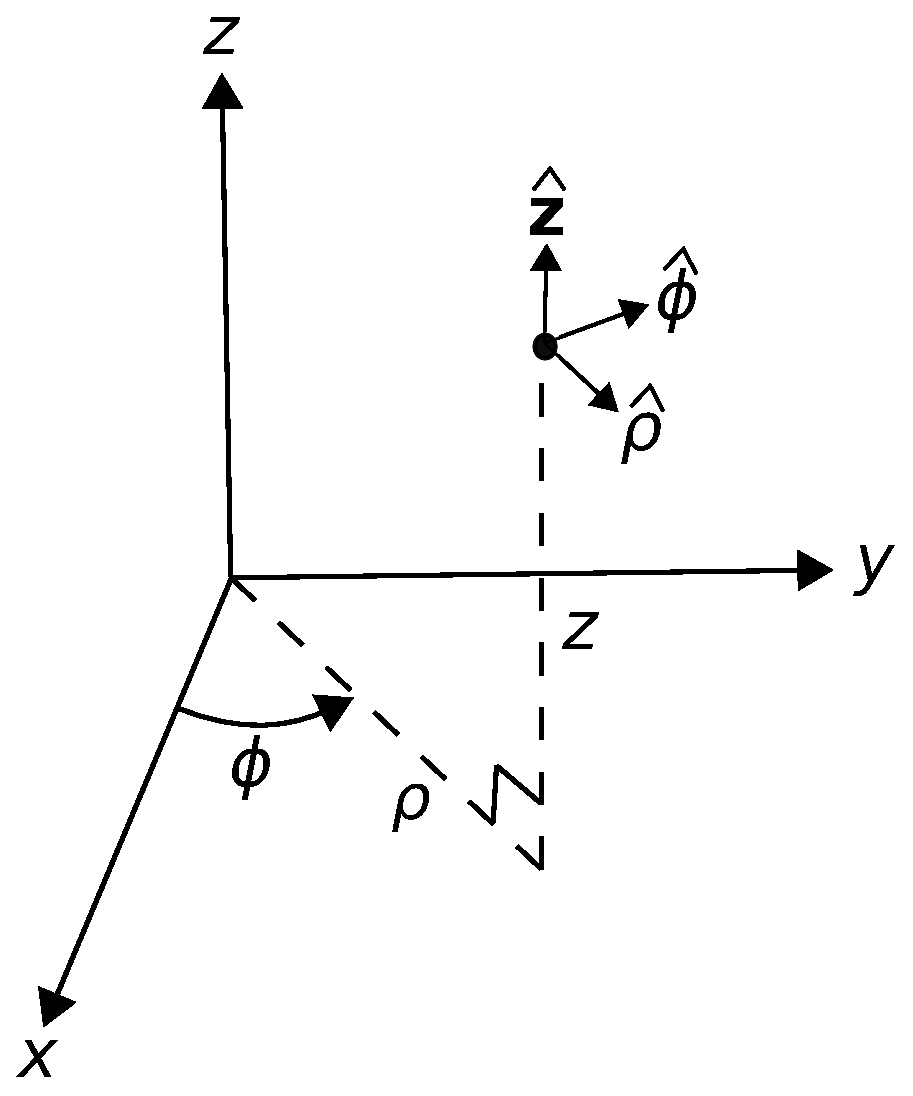
\includegraphics[width=2in]{modules/m0180_fCylindricalCoordinates.eps}
% https://commons.wikimedia.org/wiki/File:M0096_fCylindricalCoordinates.svg
}}{Cartesian coordinate system with a point arbitrarily plotted in the positive x, y, and z axes. A dashed line in the xy-plane labeled rho indicates the point’s distance from the z-axis and is shown at an angle phi from the x-axis. Another dashed line labeled z is perpendicular to rho, extends vertically from the xy-plane, and connects to the plotted point. The point has vector z-hat pointed in the z-direction. rho-hat points away from the origin, parallel to rho. phi-hat is perpendicular to z-hat and rho-hat.}
\end{center} 
\centerline{\scriptsize 
\copyright~\hyperref[m0180_fCylindricalCoordinates_Credit]{K.\ Kikkeri} 
\href{https://creativecommons.org/licenses/by-sa/4.0/}{CC BY~SA 4.0} 
} 
\caption{
\label{m0180_fCylindricalCoordinates}
Cylindrical coordinate system.
}
\end{figure}
%
\begin{figure}
\begin{center}
\pdftooltip{{  % note double braces
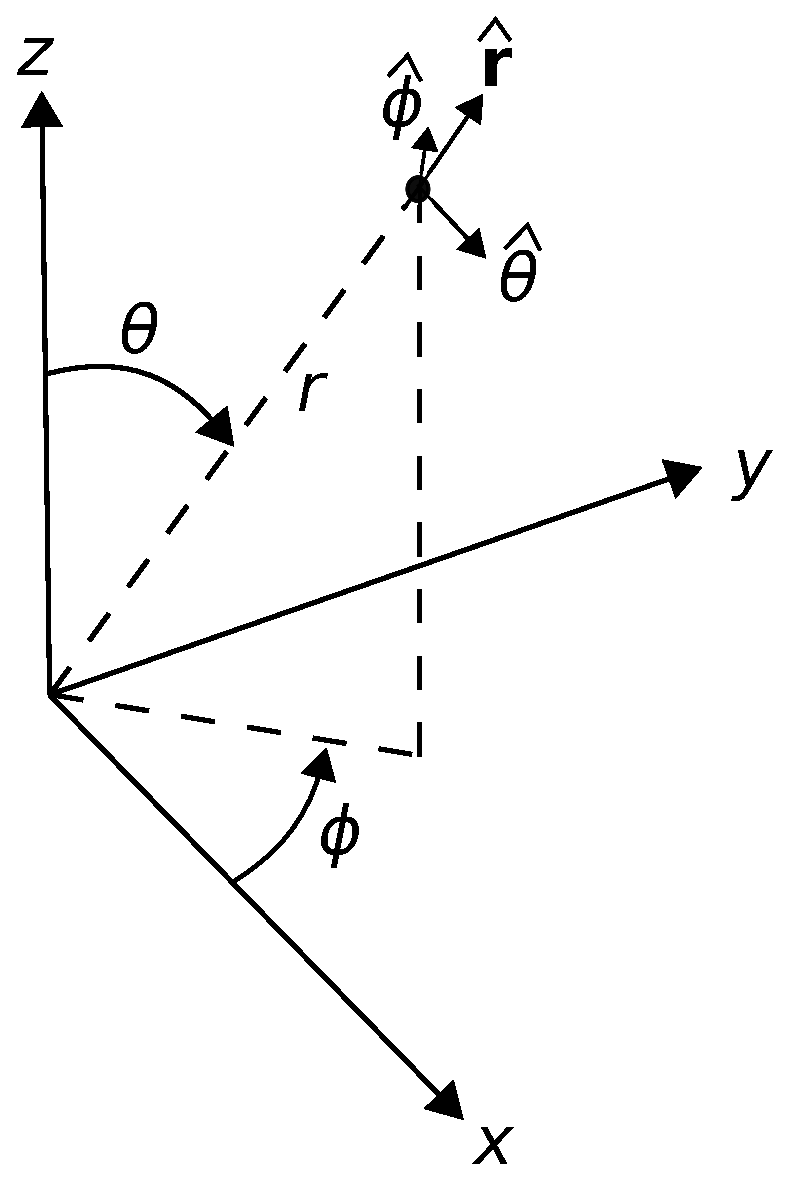
\includegraphics[width=2in]{modules/m0180_fSphericalCoordinates.eps}
% https://commons.wikimedia.org/wiki/File:Spherical_Coordinate_System.svg
}}{Cartesian coordinate system with a point arbitrarily plotted in the positive x, y, and z axes. A dashed line forms an acute triangle with one point at the origin of the Cartesian coordinate system and the top point connected to the arbitrary point with hypotenuse labeled r. The angle from the x-axis to the bottom side of the triangle is labeled phi. The angle from the z-axis to the hypotenuse is labeled theta. From the arbitrary point, vectors labeled phi-hat, r-hat, and theta-hat extend. The phi-hat vector extends parallel to the z-axis. Theta-hat extends parallel to the x-axis. R-hat is perpendicular to phi-hat and theta-hat.}
\end{center} 
\centerline{\scriptsize 
\copyright~\hyperref[m0180_fSphericalCoordinates_Credit]{K.\ Kikkeri} 
\href{https://creativecommons.org/licenses/by-sa/4.0/}{CC BY~SA 4.0} 
} 
\caption{
\label{m0180_fSphericalCoordinates}
Spherical coordinate system.
}
\end{figure}

%-------------------------------------------------------

{\bf Additional Reading:}
\begin{itemize}
\item ``\href{https://en.wikipedia.org/wiki/Cylindrical_coordinate_system}{Cylindrical coordinate system}'' on Wikipedia.
\item ``\href{https://en.wikipedia.org/wiki/Spherical_coordinate_system}{Spherical coordinate system}'' on Wikipedia.
\end{itemize}

%\item ``\href{https://en.wikipedia.org/wiki/Vector_field}{Vector field}'' on Wikipedia.
%\item ``\href{https://en.wikipedia.org/wiki/Vector_algebra}{Vector algebra}'' on Wikipedia.

%\index{cylindrical coordinate system|)}
%\index{spherical coordinate system|)}
